\documentclass{article}
\usepackage[utf8]{inputenc}
\usepackage{graphicx}
\usepackage{float}
\usepackage{csvsimple}
\usepackage{amsmath}

% https://tex.stackexchange.com/a/256190/121794
\usepackage{url}
\def\UrlBreaks{\do\/\do-}
\usepackage{breakurl}
\usepackage[breaklinks]{hyperref}
\usepackage[parfill]{parskip}

\title{Wild Goose Chase}
\author{Tong Hui Kang, Wong Tin Kit, Tey Shi Ying, Mario Josephan}
\date{8 August 2021}

\graphicspath{{./images/}}

\begin{document}

\maketitle

% camera ready
\section{Abstract}

In this report, we describe our experience participating in Hungry Geese, a Kaggle Simulation competition. In each game, four geese programmed by the teams will compete with each other. Similar to the Snake game made popular in Nokia phones, the geese extends its length by eating food and dies when its head bumps into any of the snakes. The objective of each goose is to survive 200 steps with the longest length.

Our approach to the competition is to improve on a publicly shared agent AlphaGeese. AlphaGeese follows the approach of AlphaGo, which uses a neural network model with Monte Carlo Tree Search. We have tried alternate model architectures for the neural network model, but none has been proven to be better than the neural network model published on Kaggle. We have finetuned the neural network model by training it against other top rule-based agents. We have also experimented with different ways of improving the Monte Carlo Tree Search.

By using fine-tuned agents and modifying the Monte Carlo Tree Search, we have produced agents that have higher mean rating than the original AlphaGeese agents. Tentatively, we have received a 70th with a rating of 1055.3. We have received a Kaggle Bronze medal for reaching the top 100.

% Many would have played a classic Snake game in Nokia phone in the past. It was a very popular game because it was the first mobile gaming experience for many people. There is a Kaggle competition called Hungry Geese which revolves around creating bots to play in a multiplayer snake-like game. Our group would participate in this competition by utilizing reinforcement learning model.

% The goal of our participation is to be able to obtain a high score within the competition amongst other submitted agents.



\tableofcontents

\pagebreak
% HK to edit
\section{Task Description}
\label{section_task}

Hungry Geese is a Kaggle simulation game, where each participant submit agents that compete with other agents. The rating of the team is the rating of its top agent.

In Hungry Geese, the main objective of each agent, or geese, is to survive. Similar to the Snake game popularised by Nokia phones, eating food will extend the length of the geese, and bumping to any agent will result in death.

% Statement: \textbf{Training a bot to obtain a high score in the Kaggle Competition}
% \\[1em]
% There are various method in approaching this problem. Some people may try to use classical machine learning approach such as rule-based algorithm, Greedy search and Bread-first search (BFS). While those methods are more straight forward, they are not able to beat a state of the art approaches which uses reinforcement learning model. 

\subsection{Game Rules}
\label{subsection_game_rules}

% Before considering the how the model is going to look like, we need to understand the competition rules in the first place. While most of the rules follows the original snake games, there are new rules put in place to ensure that the game is fair in the competitions. Instead of snake, Hungry Geese pits multiple goose together in a single game.

The game board is of size 11 by 7. The game board wraps at the horizontal and vertical side, in other words, travelling right of a rightmost cell will return you to the leftmost cell in the same row. An example of the game board is shown in Figure \ref{figure_gameplay}.

\begin{figure}[H]
\centering
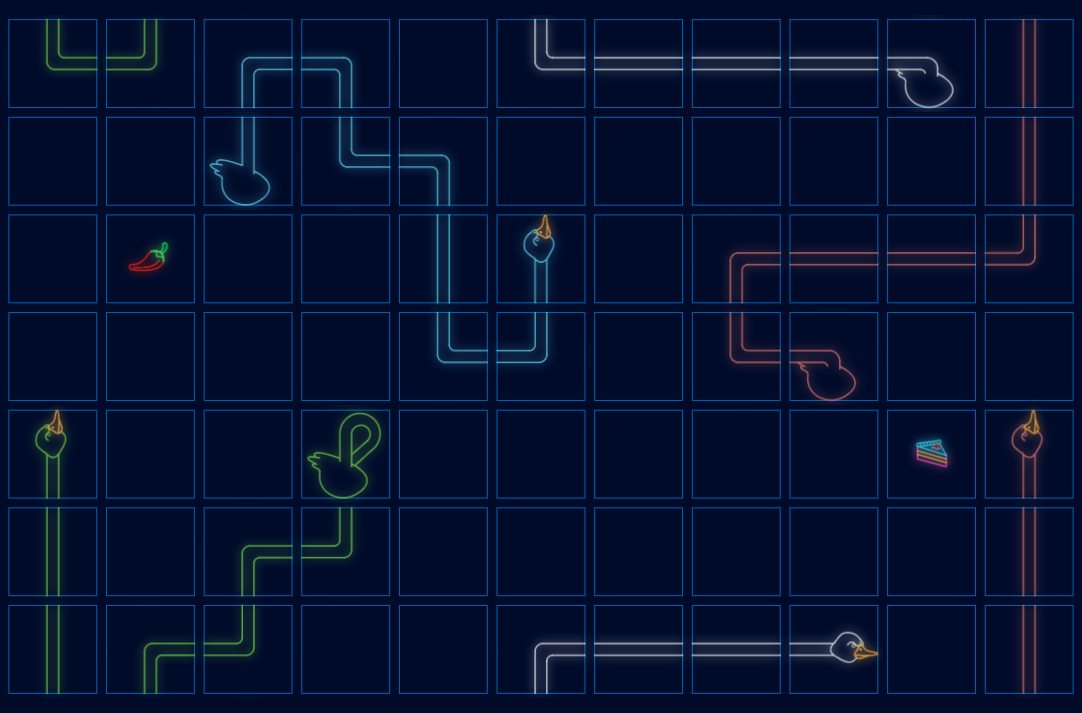
\includegraphics[width=\textwidth]{images/gameplay.png}
\caption{Gameplay Screenshot}
\label{figure_gameplay}
\end{figure}

Each goose will start with the length of one and they will spawn at a random location on the board. The game will run for a maximum of 200 turns or there is only one goose alive.

% The game board consists of 11 by 7 grid cells where each goose's body occupy a single cell \cite{game_rules}. This constrain the space in which the goose can move around. There can be up to 4 geese competing in the game. 

In each turn, each goose can choose to move up, down, left or right, relative to the orientation of the board. The goose is not allowed to take the opposite of its previous action even if the length of the goose is below three.

When the goose eats food, its length will increase by one. There is always two pieces of food on the board, and once a food is eaten, another food will spawn at a random unoccupied cell. At every 40 turns, the each goose will lose 1 segment of their body.

% During the each turn, each goose can choose to move in either NORTH, SOUTH, EAST, and WEST. They have a maximum time of 1 seconds to decide their movement. The geese can only move for 1 cell every turn and all their body parts will move simultaneously. Food such as donuts, pizza, pie or pepper will spawn randomly on unoccupied tiles. A maximum of two food can exists at any point of time. If a goose head collides with a food, it will increase its length by 1 and another food will spawn randomly. After 40 turns, all the geese will lose 1 segment of their body.

The primary objective of each goose is to survive to turn 200. Each goose is primarily ranked by the number of turns it survives. If two or more geese survive to turn 200, or die at the same time, the geese with the longer length will get a higher rank. The rank from each game will update the rating of the agent.

% If a goose's head collides with any goose's body, that goose will be eliminated and removed from the game. Also, any goose that loses their entire body will be eliminated.

% The game will end if 200 turns have passed and a score would be calculated for each goose participating. The higher the score, the better the rank of the goose's bot. The rank and the goose previous rating will determine the new rating.

\subsection{Competition Rules}
\label{subsection_competition}

The Kaggle competition started on January 26, 2021 and submission closes on July 21, 2021. Our team joined the competition late, making the first submission on June 23, 2021. Throughout the duration of the competition, each team can submit five agents every day, which will play against other agents. The team's placing in the competition is determined by the rating of the team's highest-rated agent.

Each agent will play against other agents of a similar rating. The magnitude of the change of rating will decrease as more games are played. After the close of the submissions, play between agents will continue to allow the agent rating to converge. The results are scheduled to be finalised on August 10, 2021, which is after the deadline of this report.

% No internet connection. Logs can be printed.

% Participants are also allowed to share their approaches publicly on Kaggle, in exchange for feedback and recognition.
% Somewhere in this section mention the point that you can submit the same models from another team. Teams may share their model while the submissions are still open. They do that to influence the competition to their own benefit, or for recognition with Kaggle promotion system, or to promote something else. All sharing between teams must be public.
% camera ready
\section{The Metagame and Our Approach}

\subsection{The Metagame}
\label{subsection_metagame}

Currently, there are two popular high performing agents that people have shared during the competition. They are PubHRL \cite{notebook_pubhrl} and AlphaGeese \cite{notebook_alphageese_baseline}.

\begin{figure}[h]
\centering
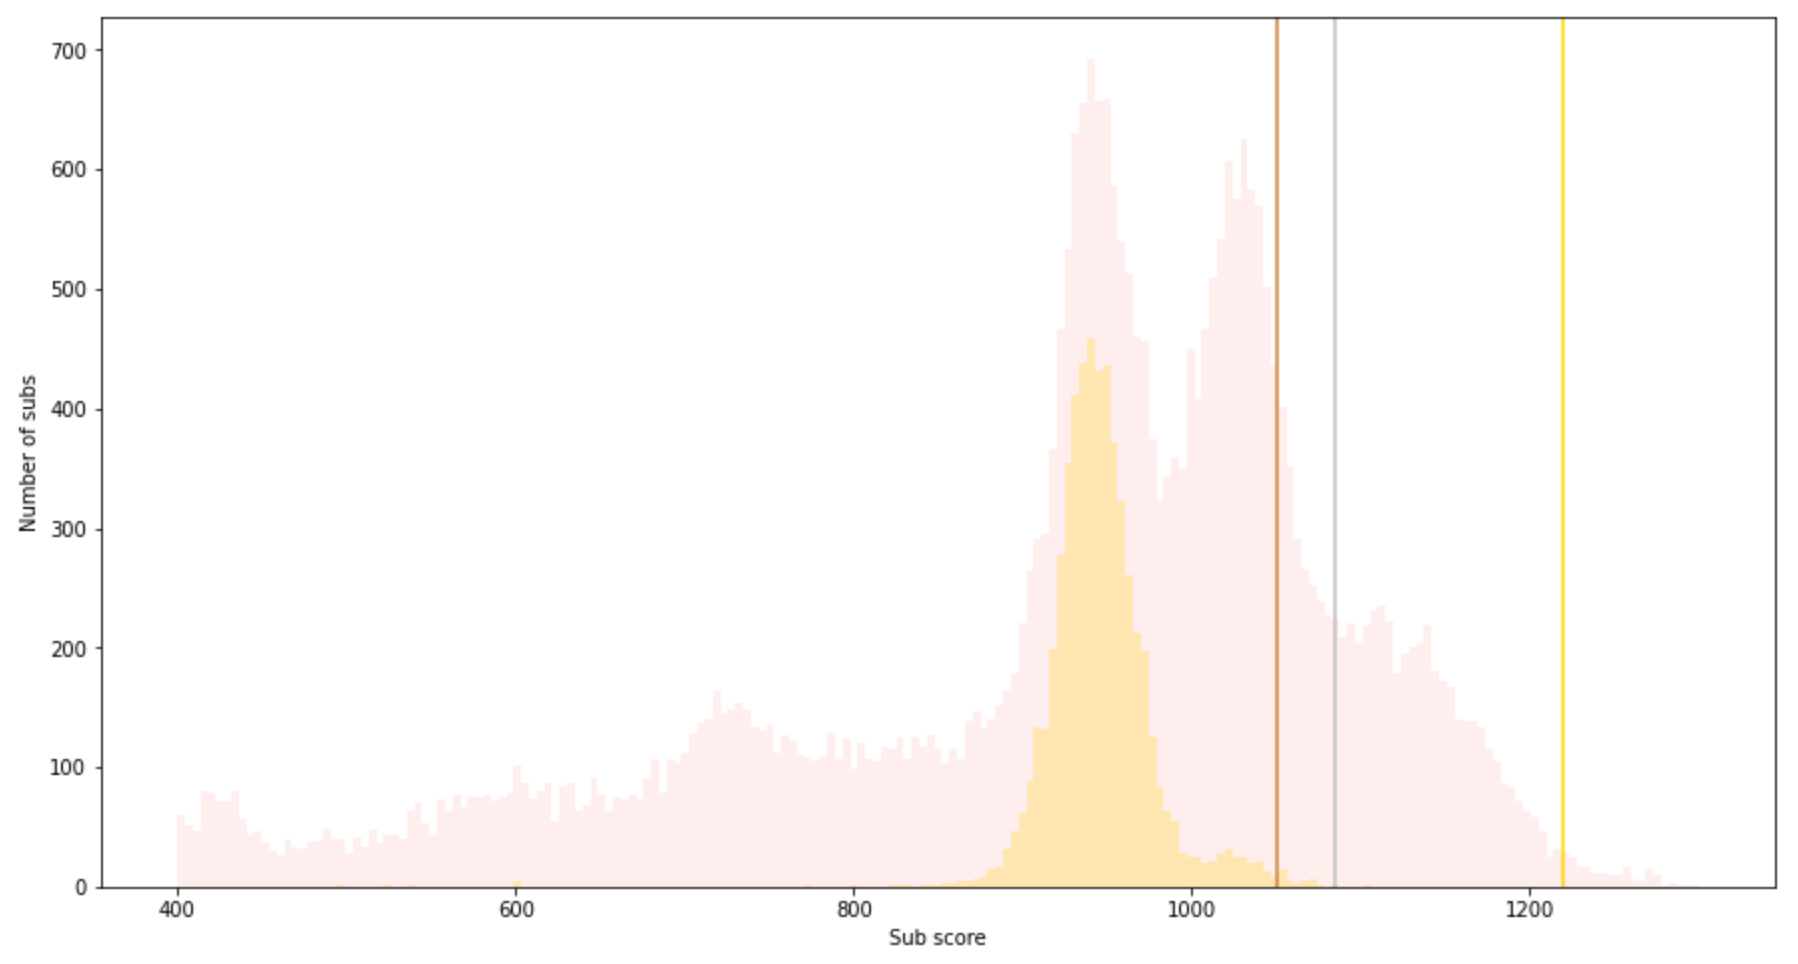
\includegraphics[width=\textwidth]{images/metagame.png}
\caption{Distribution of Scores of Submitted Agents}
\label{figure_metagame}
\end{figure}

Figure \ref{figure_metagame}, which is produced by a top participating team \cite{comment_agent_score_distribution}, shows the distribution of scores of submitted agents at the close of the submissions. The vertical lines show the required team rating to get a Kaggle Bronze, Silver or Gold medal.

The first peak is heavily contributed by PubHRL \cite{notebook_pubhrl}. PubHRL was published in February. It has been analysed that the agents shaded in yellow in Figure \ref{figure_metagame} makes moves exactly suggested by PubHRL, and the agents make up to 17.5\% of the submissions \cite{comment_agent_score_distribution}. PubHRL is a neural network model that suggest which move to take. We will elaborate on PubHRL in Section \ref{section_nn_model}.

The second peak is suspected to be heavily contributed by AlphaGeese \cite{notebook_alphageese_baseline}. AlphaGeese was published in April. AlphaGeese model uses PubHRL model inferences but it improves the performance by adding Monte Carlo Tree Search (MCTS) algorithm on top of it. This approach is similar to AlphaGo \cite{paper_alphago}, and we will elaborate this in Section \ref{section_mcts}.

\subsection{Our Approach}
\label{subsection_approach}

When we entered the competition, we have decided to improve on the best-performing approach that has been published, which is AlphaGeese. There are two aspects we can improve on AlphaGeese. One aspect is to improve the underlying neural network model in terms of performance or time, which we will explore in Section \ref{section_nn_model}. The neural network model can be improved by changing the model architecture, which we will describe in Subsection \ref{subsection_alt_model_arch_hyper_param} or changing agents it is being trained against, which we will describe in Subsection \ref{subsection_training_against_different_agents}. The other aspect is to improve how Monte Carlo Tree Search is done, which we will explore in Section \ref{section_mcts}.

Then in Section \ref{section_discussion}, we describe and analyse the results. We will also show how to set up a GUI to play against specified agents in Section \ref{section_gui}.

% Explanation of the rule-based agents? (to write?)
% The strategy of Risk Adverse Greedy Goose.



% HK to vet contributed texts
% 4.2 not written
% 4.3 onwards camera ready
\section{Neural Network Model}
\label{section_nn_model}

In this section, we first explain the input and structure of PubHRL, the neural network AlphaGeese is built upon. We explain how we attempted to improve the neural network model by changing the model architecture and the agents we train against. Finally we analyse some of the weakness of the neural network models.

\subsection{PubHRL Neural Network Model}
\label{section_pubhrl}

In this subsection, we explain the input and structure of PubHRL model \cite{notebook_pubhrl} to provide context to the improvements we attempt to make. The neural network model takes in a matrix of values, and returns four action-values and one state-value.

\subsubsection{Processing the Game State into the Model Input}
\label{subsection_pubhrl_input}

The PubHRL takes an input of a binary matrix of size (17,11,7). Each cell in the 11 $\times$ 7 game board is represented by 17 binary variables. Each "slice" of the matrix input encodes a different part of the information from the game board.

\begin{figure}[hb!]
\centering
  \includegraphics[width=0.6\linewidth]{images/input.png}
  \caption{Input block}
\end{figure}

\begin{itemize}
    \item The first four slices encode the position of the head, with one slice for each goose. The value in the matrix is 1 if the head belongs to the geese. Each slice is one-hot as there is at most one non-zero value. If the goose is dead, the slice will have values of all zeroes.
    \item The next four slices encode the position of the tail in a similar manner. Each slice of the tail encoding is one-hot.
    \item The next four slices encode the position of the body. The value in the matrix is 1 if the body belongs to the geese. These slices are not one-hot.
    \item The next four slices encode the position of the previous head position.
    \item The last slice encode the position of the food. 
\end{itemize}


% Each position the 11 \times 7 cells of each of the 17 "slice" represents the 2D positions of the game board and 17 represents the information encoded in the input. Hence, there are 17 slices of the game board that encode the different type of information from the observable data. Since there are four geese in the game, there will be four slices that encode the head, body, tail and previous head positions totaling to 16 slices. The last slice encodes the current position of the two foods. 

% This method of encoding the input is effective in transforming the observable data into a matrix form which is more suitable for deep learning model. 

There is sufficient information encoded in the input. The model can infer the length and shape of the goose from the position of the head, body and tail. Likewise, the direction of the previous move can be deduced from the difference between the position of the current head and the previous head. The input also takes into account the position of the other goose as well so that the goose can avoid colliding with them.

% The game provides all the observable information of the game environment at the current state to the agent. Information given are the exact position of the goose in the game board including the current placement of the food. Non-observable information such as where the next food is going to spawn is not given.

% discuss the merits of this encoding

\subsubsection{The Torus Block}
% to add - why the model is designed this way

The Torus Block consists of a two-dimensional convolution, ReLU and residual connections. A diagram of the architecture of the Torus Block can be seen as follows.

\begin{figure}[h!]
\centering
  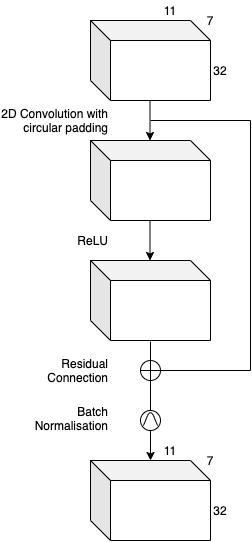
\includegraphics[width=0.4\linewidth]{images/torusblock-edit.png}
  \caption{Torus Block Architecture}
\end{figure}

The two-dimensional convolution uses filter size of 3 $\times$ 3 and has circular padding of size one to model the wrapping game board. The shape of the variables before and after the convolution is the same.

The output of the convolution is passed into ReLU. A non-linear function is used so that the neural can learn and produce a nonlinear decision boundary with non-linear combinations of the weight and inputs.

The output of ReLU is added with the input of the Torus Block. This summation is a residual connection and allows the model to address the vanishing gradient problem. In training, batch normalisation is also applied to improve gradient flow.

% is a piecewise linear function that outputs the input directly if positive, elsewise output zero. It is a favoured activation function because of its ease in calculation, and does not have a gradient vanishing. The Resnet layers create shortcut connections which control how much information from the past gets passed to the next time step. This help to train deeper models by addressing the vanishing gradient problem. 

\subsubsection{PubHRL Model Architecture}

The PubHRL model architecture is made up of Torus Blocks and fully connected layers.

\begin{figure}[h!]
\centering
  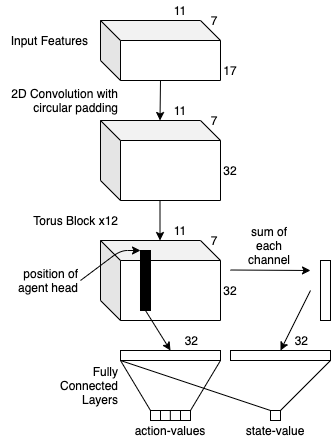
\includegraphics[width=0.6\linewidth]{images/pubhrl-edit.png}
  \caption{PubHRL Architecture}
\end{figure}

One convolution with circular padding transforms the input of size (17,11,7) to intermediate features of size (32,11,7). Then 12 Torus Blocks are applied on the intermediate features, which does not change the variable size of (32,11,7).

The values at the head position of the player's agent are extracted from the matrix, forming an array of size (1,32). The values at each of the 32 channels are summed, forming another array of size (1,32).

A fully connected layer transforms the values of the first array to the action-values. Another fully connected layer transforms the concatenation of the first and second array to the state-values. The fully connected layers are configured without bias.

This is how the model produces four action-values and one state-value. The model can be used directly to make inferences on which move to make, just by taking the action with the highest action-value.

% The PubHRL model is used to perform feature extraction based on the input data. The output is obtained in the advised next action and the resulting state value.

% The PubHRL model has 12 Torus Block Layers, in which the 32 features corresponding to a certain cell in the block is concatenated with the sum of each of 32 channels. The 64-bit value is then rearranged to output the advised next action and resulting state value.



% elaborate on the motivation behind the design on this model

\subsection{Dataset, Loss, and Training Architecture}
\label{subsection_dataset_and_training}
% HK still need to study what is going on.

As this is a reinforcement learning problem, dataset and loss functions are defined differently compared to supervised training. The objective of the training is to train the model to produce a good estimate of the policy-value and state-value.

The state-value $V^\pi(s)$ is the expected discounted return for a given state $s$ following policy $\pi$ that is assumed to be optimal. The action-value $Q^\pi(s,a)$ is the expected discounted return for taking action $a$ from a given state $s$ following policy $\pi$ that is assumed to be optimal \cite{blog_reinforcement_learning}.

As the number of possible game states is large, it is not possible to calculate the exact expectation for every state-value and action-value. Therefore state-value and action-value is approximated with a function, and the function is a neural network. The neural network is trained on squared loss \cite{blog_reinforcement_learning} between the predicted values and estimated values generated from the simulating the game.

One way to estimate the action-value and state-value without enumerating all possible states is to randomly simulate the actions until it reaches a terminal node in each complete episode. The payoff associated with the terminal node is backpropagated, thereby providing action-value and state-value for training. This method is known as the Monte Carlo (MC) method \cite{book_rl}.

It is possible to learn from incomplete episodes with Temporal Difference (TD) learning \cite{book_rl}. TD learning methods update targets with value estimates rather than solely relying on actual rewards from complete episodes as in MC methods. 

% Estimates are made with actors simulating the actions producing experience trajectories to learn from. The learner will use the experience trajectories to update the neural network parameters.
% last sentence I smoke one

It is possible to scale up training to achieve a very high throughput with the Importance Weighted Actor-Learner Architecture (IMPALA) framework \cite{paper_impala} \cite{blog_policy_gradient}. In the IMPALA framework, actors generate experience trajectories in parallel, while the learner optimizes the neural network parameters using generated experience. Actors update their parameters from the learner periodically. Because acting and learning are decoupled, we can generate many episodes with many actors in parallel and train the model more quickly. IMPALA also uses an off-policy gradient algorithm \cite{paper_off_policy} and TD learning to allow the decoupling and learning from past episodes for better sample efficiency and exploration \cite{blog_policy_gradient}.

HandyRL \cite{repo_handyrl} is an implementation of the IMPALA framework. We have used the training hyperparameters shared by PubHRL authors \cite{discussion_PubHRL_parameters}.

\subsection{Training Setup}
\label{subsection_training_setup}

The IMPALA framework allows the use of distributed computing resources to allow a high throughput for reinforcement learning training. For this to be possible, we need access to many virtual CPUs and a GPU. Therefore, we have trained our models on the Google Cloud Platform. Figure \ref{figure_training_setup} shows a screenshot of our training setup.


% [to paraphrase] HandyRL is a handy and simple framework based on Python and PyTorch for distributed reinforcement learning that is applicable to your own environments. HandyRL focuses on a practicable algorithm and implementation to create a strong and winning AI in competitive games. For large scale training, HandyRL provides a controllable high parallelism power according to your environment.

% [to paraphrase] HandyRL mainly provides a policy gradient algorithm with off-policy correction. From the perspective of stability and performance, the off-policy version policy gradient works fine in practice. So it’s a good first choice to create a baseline AI model. You can use some off-policy variants of update methods (targets of policy and value) from traditional ones (monte carlo, TD(lambda)) to novel ones (V-Trace, UPGO). These items can be changed in config.yaml.

% [to paraphrase] As a training architecture, HandyRL adopts a learner-worker style architecture like IMPALA. The learner is a brain of training which updates a model and controls the workers. The workers have two roles. They asynchronously generate episodes (trajectories) and evaluate trained models. In episode generation, self-play is conducted as default.

% [to paraphrase] In order to scale up RL training to achieve a very high throughput, IMPALA (“Importance Weighted Actor-Learner Architecture”) framework decouples acting from learning on top of basic actor-critic setup and learns from all experience trajectories with V-trace off-policy correction.

% [to paraphrase] Multiple actors generate experience in parallel, while the learner optimizes both policy and value function parameters using all the generated experience. Actors update their parameters with the latest policy from the learner periodically. Because acting and learning are decoupled, we can add many more actor machines to generate a lot more trajectories per time unit. As the training policy and the behavior policy are not totally synchronized, there is a gap between them and thus we need off-policy corrections.

% [to paraphrase] The underlying idea is that over time, the network will learn what states eventually lead to wins (or losses). In addition, learning the policy would give a good estimate of what the best action is from a given state. The neural network architecture in general would depend on the game

\begin{figure}[h]
\centering
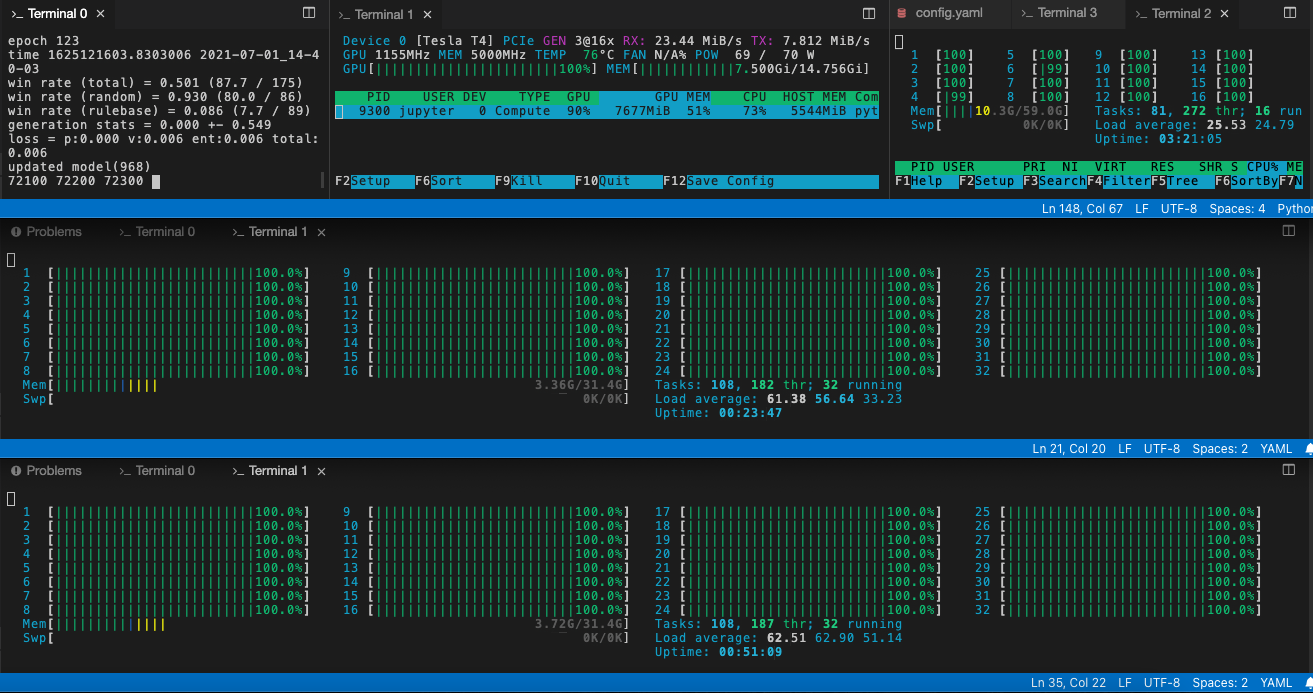
\includegraphics[width=\textwidth]{images/training-resources.png}
\caption{Screenshot of Training Setup}
\label{figure_training_setup}
\end{figure}

The actors are run on two preemptible \verb|e2-highcpu-32| instances. As the actors do not require much memory, a \verb|highcpu| instance subclass is chosen for some cost savings. As training is decentralised, the instances are also preemptible to save up to 80\% of the cost. The actors cost around US\$0.71 per hour.

The learner is run on one \verb|n1-highmem-16| instance with a T4 GPU. We need a instance with high memory to store the large number of episodes for experience replay. The instance will cost around \$1.30 per hour \cite{website_google_compute_engine_pricing}.

It takes 24 hours to train the PubHRL model with 2.1 million generated episodes over 4200 epochs. The training curve is shown in Figure \ref{figure_alt_arch}. The \$300 Google Cloud welcome credits has helped to alleviate our computation costs.

\subsection{Alternate Model Architectures and Hyperparameters}
\label{subsection_alt_model_arch_hyper_param}

Modifying the model architecture has the potential to improve the model. A model can be considered to have improved if it provides better suggestions on which move to take, or takes a shorter time to make an inference.

There is a performance-cost trade-off when we design the model architecture. A larger model may have a better performance, however, a larger model takes a longer time for inference. The larger model with a better performance may not produce a better agent as the depth of the tree search is shallower. 

This section documents the different model architectures that we have tried. Figure \ref{figure_alt_arch} shows the training curve against the default rule-based agent by Kaggle \cite{repo_kaggle_environments}. The objective function value is defined to be 1.00 if the model gets a first place, 0.67, 0.33 and 0.00 if the model gets second, third or fourth place. The score plotted is the average of the 500 games simulated per epoch.

\begin{figure}[h!]
\centering
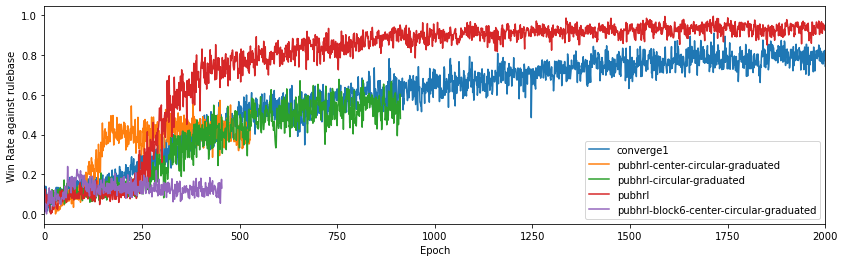
\includegraphics[width=\textwidth]{images/model-variations.png}
\caption{Training Trajectories of Various Models}
\label{figure_alt_arch}
\end{figure}


\verb|pubhrl|\newline
We attempt to reproduce the training with the original model architecture shared by HandyRL. We use the training hyperparameters shared by the authors \cite{discussion_PubHRL_parameters}.
Notably, the performance of the model only start to significantly improve after the 250th epoch. This suggests the volatile nature of training reinforcement learning models.

\verb|pubhrl-circular-graduated|\newline
In the input to the original model, the orientation of the body is not well-defined. The main change in this variant is to modify the input to better define the orientation of the body. Instead of having binary input for the four body slices, we used \verb|2/math.log(i,2)| where \verb|i| is $4$ if it is the tail, and an increment for every unit of body from the tail. The tail will have a value of $1$, and it decreases asymptotically to zero further away from down the tail. The intention is to encode the arrangement of the body in the hopes that the model will learn the arrangement. A high value implies that the location will soon be unoccupied.

We also changed the code that builds the convolutional layers, even though the behaviour is the same. The original PubHRL code makes copies of the array to pad feature matrix. We avoided the copying by using PyTorch \verb|nn.Conv2d| with the initialisation parameter \verb|padding_mode| as \verb|"circular"|.

\verb|pubhrl-center-circular-graduated|\newline
In addition to the previous model, we transpose the input such that the head is always at the coordinate \verb|(0,0)|. While we a steep improvement in training objective score at the at around the 100th epoch, the performance plateaued.

\verb|pubhrl-block6-center-circular-graduated|\newline
In addiditon to the previous model, we attempt to train a smaller model and see if is possible to achieve comparable performance. The original model architecture has 12 layers of Torus Blocks, we have reduced to 6 in this experiment. However, we have given up on the training as we do not see the model performance improve at the 400th epoch.

\verb|converge-1|\newline
This model architecture is inspired by the ResNet architecture \cite{paper_resnet}. After every residual block the the ResNet, a pooling operation is applied which reduces the dimension while increasing the number of channels. This allows more abstract features to be learnt. While the training trajectory is promising, it does not perform better at the training objective.

The alternate model architectures we have experimented did not produce superior performance on the training objective compared to the original model shared by the authors. Therefore, in our future experiments, we continued used the original architecture. After the competition, one of the top teams reported that drastically different models, such as multi-layer perceptrons and minified versions of ResNet and EfficientNet, have not shown benefit  \cite{sharing_robga}.

\subsection{Training against Different Agents}
\label{subsection_training_against_different_agents}

Instead of modifying the model architecture, there is an opportunity to improve the performance of the model by changing the agents that the model is trained against. In the Figure \ref{figure_alt_arch}, the model is trained against the default rule-based agent provided by the repository. In this subsection, we trained the model against better rule-based agents shared by other participants on Kaggle. The training logs and the code to plot the logs are available in an repository described in Section \ref{subsection_training_logs}.

As we use the same model architecture as PubHRL shared by the HandyRL authors, we begin our training from their pretrained parameters.
\newline

\begin{figure}[h!]
\centering
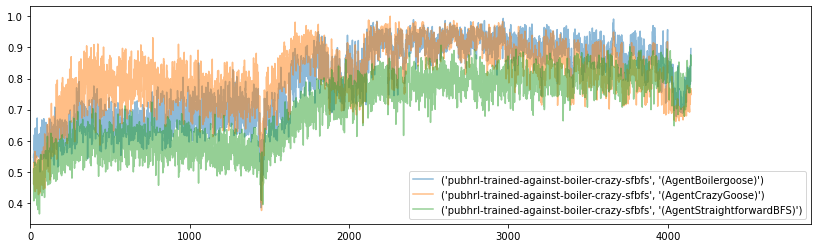
\includegraphics[width=\textwidth]{images/model-against-boiler-greedy-bfs.png}
\caption{Training Trajectories against three rule based agents}
\label{figure_assorted}
\end{figure}


\verb|pubhrl-trained-against-boiler-crazy-sfbfs|\newline
We finetune the PubHRL parameters by training against three agents - namely 
Boilergoose \cite{notebook_boilergoose}, Crazy Goose \cite{notebook_crazy_goose} and Straightforward BFS \cite{notebook_agents_comparison}. These three agents are selected from because their general good performance against other rule-based agents and against PubHRL \cite{notebook_agents_comparison}. 

The trajectory of the training objective is plotted in Figure \ref{figure_assorted}. As we use the pretrained parameters, the training objective value starts at around 0.5, rather than zero when trained from scratch. There is an unexplained dip in training objective value at around 1500th epoch, after which the model improved its performance to some peak. However, at the end of training, the training objective value declined.

\begin{figure}[h!]
\centering
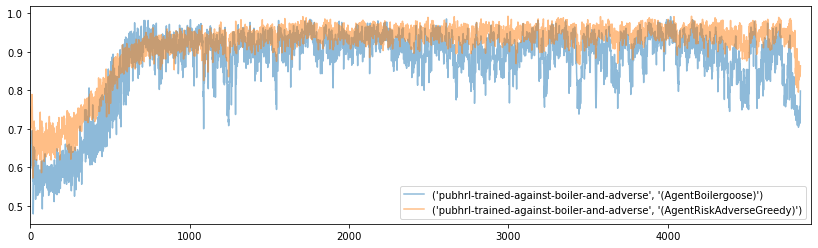
\includegraphics[width=\textwidth]{images/model-against-greedy-adverse.png}
\caption{Training Trajectories against two rule based agents}
\label{figure_greedy_adverse}
\end{figure}

\verb|pubhrl-trained-against-boiler-and-adverse|\newline
We decide the reduce the number of agents that we are training against. We choose to train the model against Boilergoose \cite{notebook_boilergoose} and Risk Adverse Greedy Goose \cite{notebook_risk_adverse_greedy} because of their very different strategies but similarly high performance. We managed to train the model to score at around 0.9 against both models. After 4000 epochs, the training objective value declined. Eventually, we used the model checkpoint at the 3600 epoch.


\subsection{Weaknesses of the Neural Network Model}
\label{subsubsection_nn_weakness}

The neural network may produce suggested moves that are certain to be bad. We show two examples from the neural network fine-tuned by us.

\subsubsection{Tail Strike}
\label{subsubsection_tail_strike}

It is usually permissible to enter the location of the tail of another geese, because the location is unoccupied as the other geese moves to the next step. However, if the other geese happens to capture a food in the next step, the location of the tail is not unoccupied. This results in the elimination of the geese. Due to the rarity of such occurrence, the model might not be able to train on this scenario well enough.

\begin{figure}[h!]
\centering
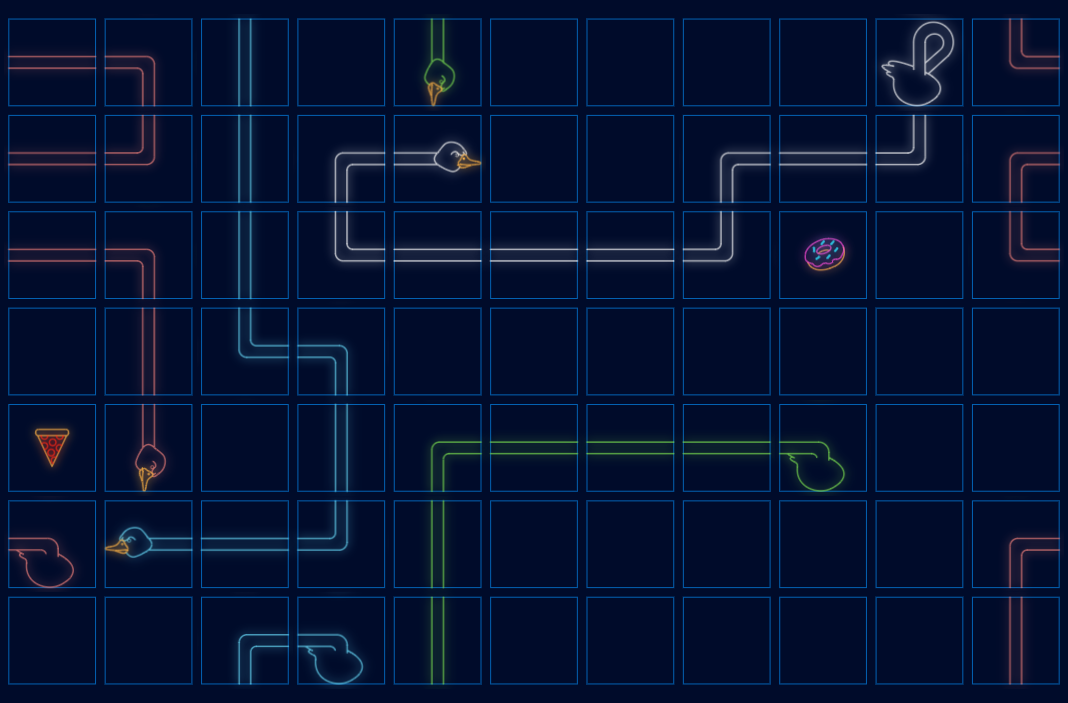
\includegraphics[width=\textwidth]{images/scenario-tail-strike.png}
\caption{Scenario of Tail Strike (Our agent is blue)}
\label{figure_tail_strike}
\end{figure}

Figure \ref{figure_tail_strike} shows a scenario of a tail strike. Our agent blue, is considering two feasible moves, left or down.

\begin{table}[h!]
\begin{tabular}{lllll}
Direction                   & Up     & Down   & Left   & Right  \\
Model Inference Probability & 0.0000 & 0.0431 & 0.9569 & 0.0000
\end{tabular}
\end{table}

In this scenario, the model make a strong suggestion to step into the location of the tail of probability 0.9569. However, the only move that red agent can make to survive is to go left to eat the food. If we follow the action suggested by the model, our agent will be eliminated.

\subsubsection{Length Ignorance}
\label{subsubsection_length_ignorance}

When two heads collide, both geese will be eliminated at the same time. The geese with the longer length will get a higher position, while the geese with the shorter length will be relegated to the lower position. However, surviving geese will be ranked better than the pair of geese which collided head-on.

\begin{figure}[h!]
\centering
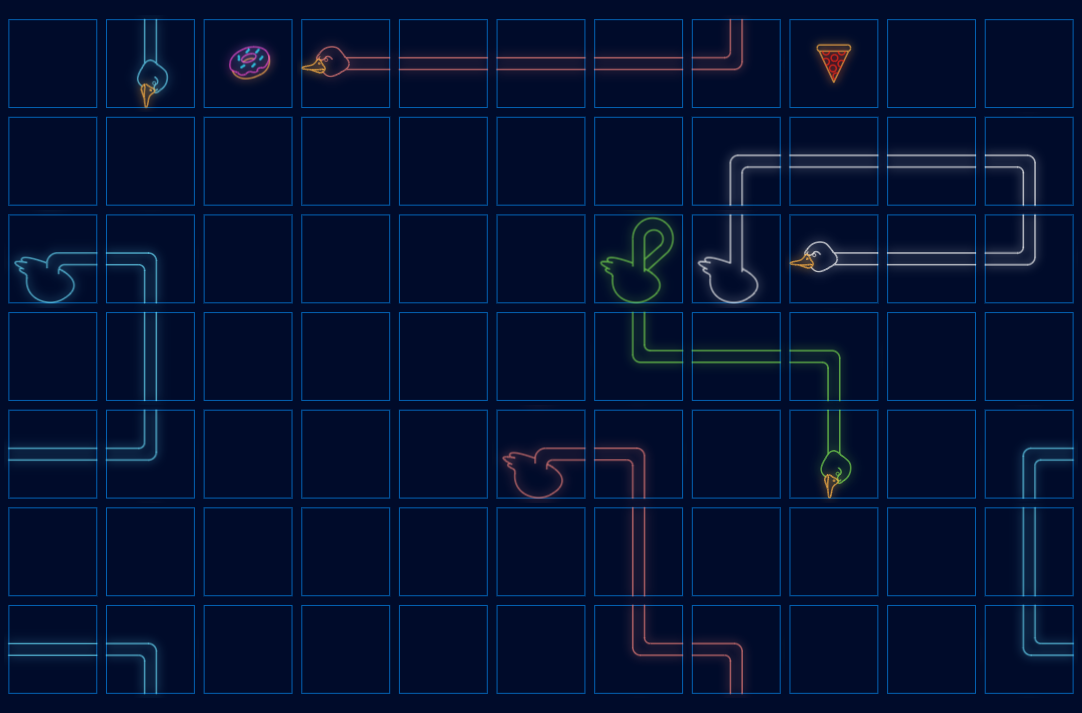
\includegraphics[width=\textwidth]{images/scenario-length-ignorance.png}
\caption{Scenario of Length Ignorance (Our agent is red)}
\label{figure_length_ignorance}
\end{figure}

Figure \ref{figure_length_ignorance} shows a scenario of a length ignorance. Our agent red, is considering three feasible moves. The agent can move left to capture the food, or move up or down to avoid the food. Our red agent is 10 units long, one unit shorter than our rival which is 11 units long. If we collide with the blue agent over the food, we get the worst possible outcome.

\begin{table}[h!]
\begin{tabular}{lllll}
Direction                   & Up     & Down   & Left   & Right  \\
Model Inference Probability & 0.0007 & 0.0031 & 0.9962 & 0.0000
\end{tabular}
\end{table}

Neural Network models may also make other move suggestions that may result in the worst possible outcome. A top team \cite{sharing_robga} shared about how they use rule-based oversight to avoid getting into traps and corridors, as well as trapping other agents.


% random rollouts?

% We tried to self train but it does not really work. 
% camera ready
\section{Monte Carlo Tree Search}
\label{section_mcts}

As described in subsection \ref{subsubsection_nn_weakness}, the neural network model may not always provide the best action-values. This can be addressed by simulating multiple steps of the game to improve the quality of move suggestions.

The simulation is considered a tree search as we consider the possible moves made by each agent simultaneously. Each board state can be considered as a node. A directed edge between two nodes exists $i \to j$ if there is a set of valid actions from each agent that can cause a transition from state $i$ to state $j$.

As there is a maximum of four agents each making either of three possible moves, the branching factor of the game tree is 81. The branching factor is likely to decrease on average as the game progresses due to lesser geese and more crowded board space.

An exhaustive tree search is not possible due to the number of steps in the game (up to 200) as well as the large branching factor of 81. Therefore the original AlphaGeese agent uses a Monte Carlo tree search (MCTS) as a heuristic tree search algorithm. In the pure MCTS algorithm, random rollouts were made until a terminal state is reached, and what follows is the backpropagation of the payoff in the game tree. However, as it is possible for the game to progress until step 200, random rollouts are inefficient and ineffective. AlphaGo replaces the random rollouts with a neural network that infer the expected payoff at each non-terminal state \cite{blog_alphago_tutorial}. 

% In Monte Carlo Tree Search, we expand the search tree based on the random sampling of the search space. We conduct many rounds of tree search, which is called playouts. In each playout, we select moves at random and complete each game. The final outcome of each playout is used to weigh the nodes in the game tree so the better nodes are more likely to be chosen in future playouts.
% \\[1em]
% In the game, we have four actions, hence we model each node in the tree to have four child nodes, with each child node corresponding to probability of adopting a certain policy.

% As seen in Section X, the use of Monte Carlo Tree Search on top of the PubHRL makes the model superior to PubHRL.

% How concepts from game tree search can apply.

\subsection{Algorithm Implemented by AlphaGeese}
\label{subsection_alphageese_algo}

AlphaGeese \cite{notebook_alphageese_baseline} follows an implementation of MCTS \cite{repo_MCTS} \cite{paper_othello}. The implementation of MCTS tracks the following variables.

\begin{itemize}
    \item $P(s,a,i)$ The prior probability agent $i$ of taking an action $a$ from a state $s$ according to the neural network. This is the softmaxed value of the action-values inferred by the neural network.
    \item $N(s,a,i)$ The number of times we explore the action $a$ taken by agent $i$ from a state $s$ when we are searching the tree.
    \item $Q(s,a,i)$ The expected reward for taking the action $a$ by agent $i$ from a state $s$. This is initialised with the state-value inferred by the neural network. $Q(s,a,i)$ is the average of the state-values of the explored nodes in its subtree.
\end{itemize}

The action with the highest upper confidence bound $U(s,a)$ is explored.

$$
U(s,a,i) = Q(s,a,i) + c_{cpuct} P(s,a,i) \dfrac{\sqrt{\sum_b N(s,b,i)}}{1 + N(s,a,i)}
$$

Different implementations of MCTS may have different expressions for the upper confidence bound. The constant $c_{cpuct}$ is a search hyperparameter that controls the degree of exploration.

At every unexplored node, the neural network makes an inference providing the state-value and the action-values. The state-value is backpropagated in the search tree, updating $Q(s,a,i)$. If the unexplored node is a terminal state where the agent is eliminated or the game reaches 200 moves, the actual reward is backpropagated instead. The action values are softmaxed and stored as $P(s,a,i)$.

At the root node $s'$, the most explored action $\max_{a} N(s',a,0)$ is the returned result of our search strategy.


\subsection{Approaches at Improving the Search}
\label{subsection_mcts_improvements}

In this section, we describe how we attempt to improve the search and the intention behind the improvements. The code is described in Section \label{subsection_code_submission}. In the following section, Section \ref{section_discussion}, we describe and interpret the results.

\subsubsection{V13 - Use of Different Agents in Search}
\label{subsubsection_v13}

In the original AlphaGeese notebook, the PubHRL model is used to make model suggestions at every node. We replaced the pretrained parameters shared by HandyRL with our finetuned parameters.

To better simulate the opponent moves, when we are making a neural network inference for opposing agents, we use the original PubHRL parameters. This approach gave our first agents that perform better than the original AlphaGeese.

\subsubsection{V14 - Assuming Rivals follow PubHRL Deterministically}
\label{subsubsection_v14}

In the MCTS, we assume that our opponents' moves are deterministic and follow the inferences of PubHRL without modification. As this reduces the branching factor, we are also able to search more deeply into the tree. This is done by setting the setting exploration constant of other agents to zero.

\subsubsection{V17 - Use of Overage Time to Tie Break}
\label{subsubsection_v17}

Each agent is given one second to make an inference for every move. However, there is one fine detail of this rule - each agent is allowed to exceed one second for a total of one minute in each game. The original AlphaGeese model does not make use of this overage time.

One way to use the overage time is to extend the allowed duration of each move by 0.3 seconds on average. We have decided to use this overage time more strategically by spending it on moves where are current probabilities are close.

In our implementation, each move is allowed to use an overage time of up till the four times the remaining overage time if shared equally by remaining steps. We employ the overage time if the current tree search probability is under a certain threshold. As move probabilities usually increase as the board gets more crowded, the threshold is set to be 0.5 at the start, which linearly increases to 0.9 at move 200. To allow sufficient time to make the remaining moves, we do not use overage time if the remaining overage time is less than 10 seconds.

\subsubsection{V32 - Soft Masking of Undesirable Moves}
\label{subsubsection_v32}

As described in Subsections \ref{subsubsection_tail_strike} and \ref{subsubsection_length_ignorance}, the neural network may provide bad inference in certain scenarios. In an extreme case, the model may produce a probability very close to one for a move that is certain to result in the worst possible outcome.

We multiply the action-values produced by the neural network model with the following coefficients if the scenarios apply. The values of the coefficients are arbitrarily chosen.
\begin{itemize}
\item 0.000 if the move is illegal. This is already present in the original AlphaGeese notebook \cite{notebook_alphageese_baseline}.
\item 0.101 if the move results in a potential tail strike as described in Section \ref{subsubsection_tail_strike}.
\item 0.111 if there is a potential of a head collision with another goose of greater length as described in Section \ref{subsubsection_length_ignorance}.
\item 0.888 if the move results in a head collision with another goose of shorter or equal length while there are at least three remaining agents in the game.
\item 3.333 if there is are only two remaining agents in the game and you are the longer goose. In this case, a head collision secures first place.
\end{itemize}

This modifies the value of $P(s,a,i)$, which is obtained after softmaxing the action-values. We hope that this encourages the MCTS to start the search from a more reasonable, in the hopes that it will return a better result.

% camera ready, but values need to be updated
% 6.2 can be extended if applicable
\section{Results and Discussion}
\label{section_discussion}

\subsection{Agent Performance and Analysis}
\label{subsection_results}

Table \ref{table_scores} shows the performance of our agents on the leaderboard. The version refers to the notebook version. The count refers to how many of the same agents have we submitted. The mean, standard deviation and maximum ratings of the agents submitted are also tabulated. The number of wins of the agent against three copies of the original AlphaGeese agent over 100 matches is recorded under column AG.

% Table to be updated
% To compute win rate against AlphaGeese

\begin{table}[hbt!]
\begin{tabular}{lllllll}
\textbf{Model}                & Ver & Count & AG & Mean          & Std  & Max           \\
AlphaGeese without edits      & 1   & 35    & 26 & 1022          & 12.5 & 1050          \\
Use Finetuned Agent           & 13  & 11    & \textbf{35} & 1024 & 16.5 & 1045          \\
Assume Deterministic Rivals   & 14  & 10    & 28 & \textbf{1036} & 12.2 & \textbf{1055} \\
Use Overage Time to Tie Break & 17  & 8     & 25 & 1033          & 12.7 & 1054          \\
Softmasking Dangerous Moves   & 32  & 8     & 30 & 998           & 22.9 & 1022         
\end{tabular}
\caption{Comparison of Submitted Agents}
\label{table_scores}
\end{table}

The performance distribution of AlphaGeese closely matches the second peak illustrated in Figure \ref{figure_metagame}. Notably, submitting sufficient copies of AlphaGeese \cite{notebook_alphageese_baseline} can bring the participant a very good chance at winning a  Kaggle Bronze medal, which requires a cutoff of 1050 (to be determined).

The model with the best mean rating is Version 14 that assumes that the opponent is deterministic. At the close of submissions before the scores are allowed to converge further, copies of this agent has a small standard deviation in rating. The high mean and low variance score might be due to its consistent superior performance against the PubHRL submissions, while under-performing against better agents also due to the same absolute assumption of its rivals.

While our scores converge, our best agent frequently rotates between Versions 1, 13, 14 and 17. Version 14 and Version 17 has a higher and similar mean score and it expected that they deliver our top agent. Version 1 and Version 13 has a lower mean score, but is still our top agent at times. For Version 1, this is because we submitted many of its copies than the other. For Version 13, this is because the standard deviation of its rating is higher.

Regrettably for Version 32, soft-masking dangerous moves produces an agent worse than the original AlphaGeese agent. While the soft-masking addresses scenarios where the neural network model performs badly, encouraging more alternate moves may result in shallower search depth. 

\subsection{Survey of Top Performing Strategies}
\label{subsection_survey_of_top_performers}

This section summarises the successful strategies shared by the top participants. These strategies were shared when the submissions for the competition closed. 

\subsubsection{Imitating the Top Agents}
\label{subsubsection_imitation}

Match replays of submitted agents are publicly available \cite{notebook_scraper}. A model can be trained by learning the moves of top-rated models. The score of models trained by imitation learning is reported to be rated at around the mid-1100s, which is more than sufficient for a Kaggle Sliver medal \cite{sharing_robga}. The AlphaGeese author used the same PubHRL model architecture but trained with imitation learning obtained a score very near the Kaggle Gold medal boundary \cite{notebook_alphageese_imitation}.

\subsubsection{Optimising Model Inference Speed}
\label{subsubsection_speedup}

One top participant \cite{sharing_robga} exported the PyTorch model into and an ONNX Runtime. ONNX Runtime parses the model to identify optimization opportunities and provides access to the best hardware acceleration available \cite{website_onnx}. The optimisation has improved the model inference time from 3.42 milliseconds to 0.77 milliseconds \cite{sharing_robga}. By improving model inference times by approximately four times, it is possible to search four times as many more nodes and allow a better performance without any tradeoff.

\subsubsection{Differentiating the Agent Behaviour}
\label{subsubsection_time_diff}

While the agents are denied internet connection, the agents have access to the system date and time. It is possible to program the agent to have different behaviour after a predefined time. 
One top participant \cite{sharing_robga} implemented a 90-minute timer so that when the agent is competing with lower-ranked agents right after when the agent is submitted, the agent will not make risky moves. This submission strategy is in response to the observation that agents rated below 1000 can make dangerous moves. This helps the agent to climb the ratings quickly.

As observed in Table \ref{table_scores}, our agents have a different standard deviation in ratings even though their mean is similar. There is a possibility that some of our agents perform better at higher ratings if given a chance to reach the rating band.

The extension to this idea is for the agent to use a fake strategy until the close of submissions. This way, the team can submit more duplicate agents for a better chance at a higher maximum rating, while reducing imitation attacks.

\subsubsection{Building an Evaluation System}
\label{subsubsection_eval}

Another popular practice of top teams is to implement a systematic procedure to benchmark their agents. Submitting the agent into the competition is the most convenient method of getting accurate feedback for how well the agent is performing. However, each team can only submit up to 5 agents each day, and it will take around a day to converge to a stable score. The stable score it converges to will still have a large standard deviation. Moreover, submitting your agent onto the leaderboard leaves the agent prone to imitation by other competitors.

The evaluation system implemented by top teams is similar to how we evaluate our agents against the original AlphaGeese agent as describe in Subsection \ref{subsection_results}, but at a larger scale and in parallel. Some teams went on to implement their own "league of agents" to estimate the rating of their agents \cite{sharing_ironbar}. A robust and efficient evaluation system will allow more variants of agents to be developed and tested.

% \subsubsection{Training on Different Game Rules}
% \label{subsubsection_diff_rules}

% There are some ideas that we have after the close of the submission.

% One idea is to train the model on a game with slightly different rules. In the model, the game ends at the 200th turn. Another fine rule of the game is that agents will have their length shortened by one at every 40 turns. Our suggestion is to modify these rules in training. The agent will train a board that will end its game at a probability of 1/100 after the 100th turn. Moreover, the agent will no longer shorten its length at every 40 turns. This allows the payout to be computed at every point in time.


% \subsubsection{TBC, Waiting for more top participants to share}

% TBC \cite{sharing_robga}
% TBC \cite{sharing_ironbar}


% \subsection{Takeaways for Reinforcement Learning}

% TBC

% more like awareness, rather than fighting against them
% \noindent Metagaming is a term used in role-playing games, which describes a player's use of real-life knowledge concerning the state of the game to determine their character's actions, when said character has no relevant knowledge or awareness under the circumstances. Metagaming are illustrated as strategies (ie. submitted agent models) that allow them to beat other agents. With these models, these agents will be able to leverage on the underlying Artificial Intelligence methodology to increase their performance in an adversarial setting.
% \\[1em]
% There are two very popular models in Hungry Geese Kaggle Competition


\section{Conclusion}

This is our first project at reinforcement learning and we have glad to be able to make improvements on the agents published during the competition.

There are a few takeaways for future reinforcement learning projects. It is important to start from the state-of-the-art when designing the neural network model. The PubHRL neural network model is inspired by AlphaGo, and has proven to have good performance. The time-complexity tradeoff is also needed to be considered in the design of the neural network model, as more time-consuming model will result in a shallower search. We also sense that reinforcement learning models favors simplicity in both the design of the neural network model and the Monte Carlo Tree Search. It is also important to build a validation process to conduct ablation tests on improvements that you are experimenting. If you have access to plays by the top agents, imitation learning is able to provide strong results with a simple setup. We hope these takeaways can help participants get started in future reinforcement learning projects.
% camera ready
\pagebreak
\section{GUI Setup and Demonstration}
\label{section_gui}

Following contains the steps to set up the GUI
\begin{enumerate}
  \item Clone the Github repository \newline \verb|git clone https://github.com/tinkitwong/kaggle-environments|.
  \item Navigate into directory of the repository
  \item Create a python Virtual Environment \verb|python3 -m venv env|
  \item Activate Virtual Environment \verb|source env/bin/activate|
  \item Install Dependencies \verb|pip install requirements.txt|
  \item Start the Jupyter server \verb|./env/bin/jupyter notebook|
  \item Navigate into notebook \verb|playtest.ipynb|
  \item Run the first two cells of the notebook (Figure \ref{figure_controls})
\end{enumerate}

\begin{figure}[!h]
\centering
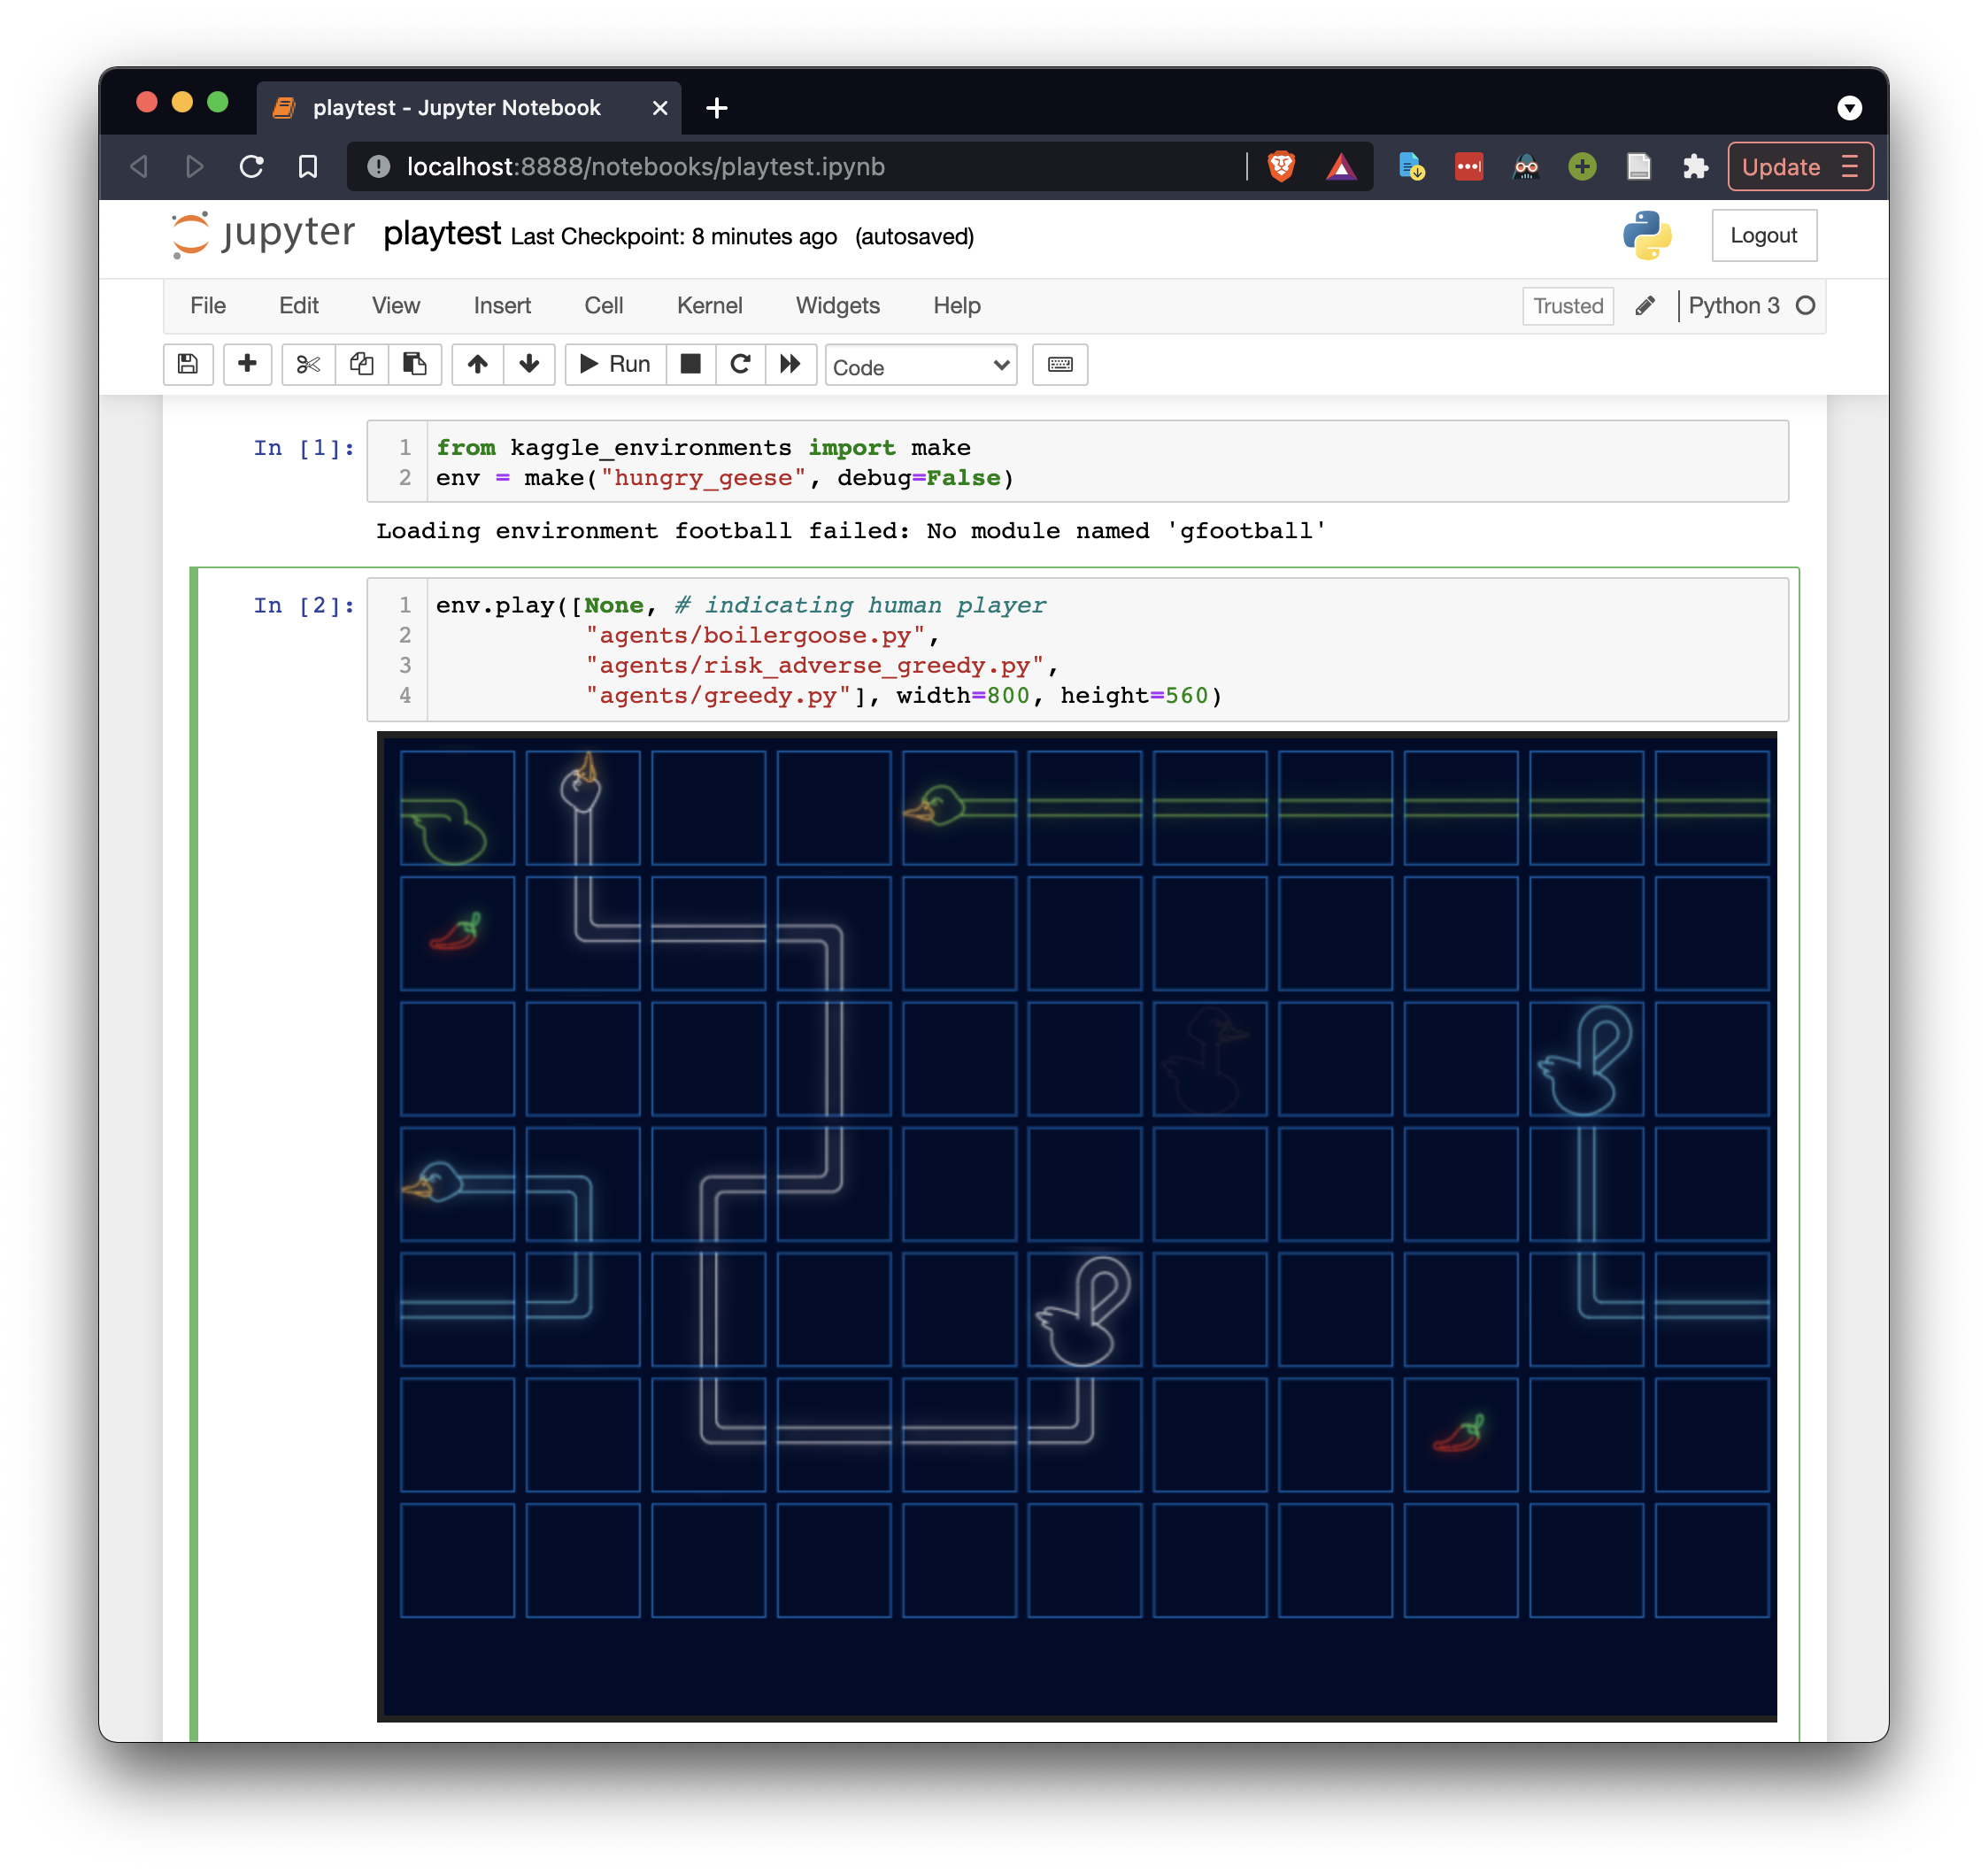
\includegraphics[width=0.95\textwidth]{images/notebook.png}
\caption{Screenshot of our GUI to play against the agents}
\label{figure_controls}
\end{figure}


% \newpage
% \begin{figure}[h]
% \centering
% \includegraphics[width=\textwidth]{images/root dir.png}
% \caption{Directory Hierachy in Jupyter Notebook after setup}
% \end{figure}

% \noindent Completing the above listed items allow you to start a local Jupyter Notebook with the local repository as the root directory as seen in Fig. X. We have provided a starter code within \verb|HumanPlayer.ipynb| illustrated in Figure 2.


When the game screen has loaded like what is seen in Figure \ref{figure_controls}, use your keyboard arrow keys (up, down, left, right) to move your agent. Your agent is the white goose.

You may choose to play against other agents by changing the arguments passed into \verb|env.play()| This list of agents are inside the \verb|./agents| folder. You may also add your own custom agent to play against. Playing against agents using Monte Carlo Tree Search is likely to be slow.

% We have configured the environment to keep playing until there is only one snake left, which would then be considered as the winner.

% \noindent Fig. X above shows the code to introduce a human player into the snake-game against other agents. To play against other types of agents, we can replace the list argument to \verb|env.play()| with a list of other agents while keeping one element as \verb|None| to represent the human player. At the moment, we only configured for 1 human player. Other types of agents are:

% %try to compress this into fewer lines?
% \begin{itemize}
%   \item \verb|boilergoose|
%   \item \verb|crazy_goose|
%   \item \verb|pubhrl|
%   \item \verb|pubhrl_latest|
%   \item \verb|risk_adverse_greedy|
%   \item \verb|simple_bfs|
%   \item \verb|simple_toward|
%   \item \verb|straightforward_bfs|
% \end{itemize}


% I have shown them together
% \section{GUI Code}
% \begin{figure}[h]
% \centering
% \includegraphics[width=\textwidth]{images/Human Player Code.png}
% \caption{Quickstart Code for Human Play}
% \end{figure}

% \begin{figure}[h]
% \centering
% 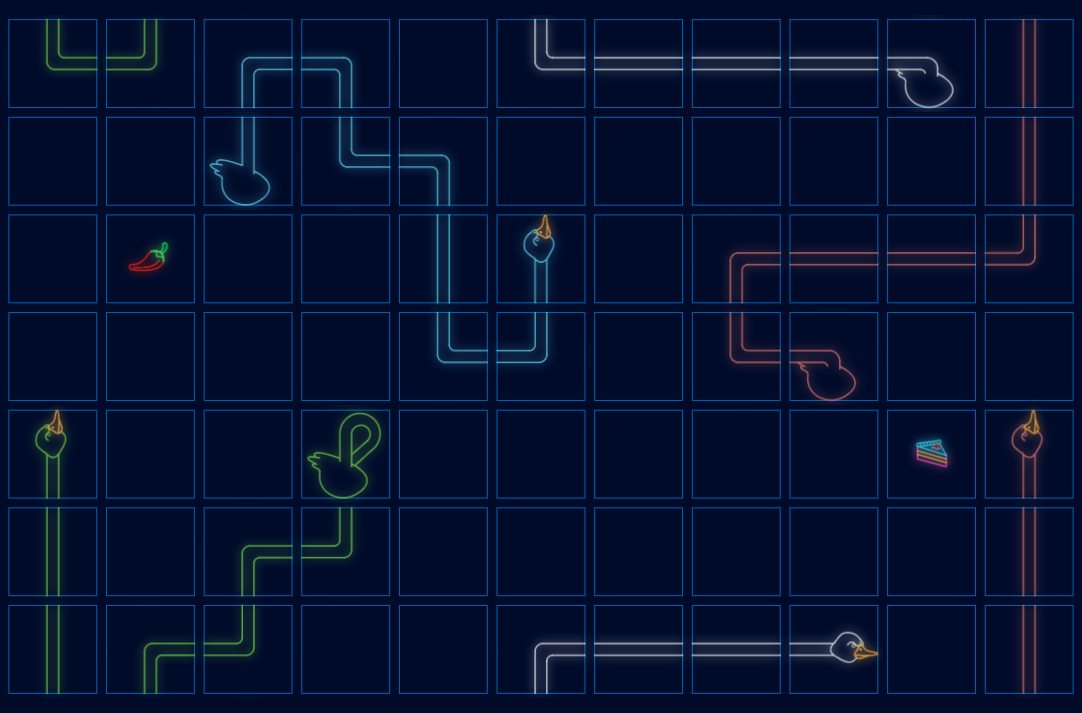
\includegraphics[width=\textwidth]{images/gameplay.png}
% \caption{Interactive Human Gameplay against loaded agents}
% \end{figure}

% \noindent Fig. X shows the step 10 of a current on-going game of a human player against 4 greedy agents. 



% camera ready
\section{Our Code}
\label{section_code}

This section documents the code that we have written for this project. Most of the code that we have used is either a fork of another repository on Github or a fork of another notebook on Kaggle. We also briefly describe the source of our code, how did we edit the code, and what the code is used for.

You may see the specific changes we made in the original versions. For Github, you can see the commit history of our forked repositories. For Kaggle, you can click on the version history of the notebooks, and compare the difference between the two versions in the history.


\subsection{HandyRL Fork}
\label{subsection_handyrl_fork}

\verb|https://github.com/tonghuikang/handyRL| \newline\newline
This repository contains the attempted edits to train the model from scratch. We attempted to train the model with different neural network architecture, or with against different agents. This repository is a fork of a distributed reinforcement learning library from the PubHRL authors \cite{repo_handyrl}.

The variations of the model architecture listed in Subsection \ref{figure_alt_arch} is recorded in different branches. The branches can be accessed here. \newline
\verb|https://github.com/tonghuikang/HandyRL/branches/all|


\subsection{Training Logs}
\label{subsection_training_logs}

\verb|https://github.com/tonghuikang/hungry-goose-training-logs/|\newline\newline
The \verb|logs/| folder contains the training logs for Section \ref{subsection_alt_model_arch_hyper_param} and \ref{subsection_training_against_different_agents}. \verb|analysis.ipynb| contains the code to make the plots in Figure \ref{figure_alt_arch}, \ref{figure_assorted} and \ref{figure_greedy_adverse}. The folder \verb|strings| contains base64 model paramters.


\subsection{Submitted Agents}
\label{subsection_submission}

\verb|https://www.kaggle.com/huikang/hg-alphageese-baseline|\newline\newline
In order to submit to the competition, you need to produce a notebook on Kaggle that generates a Python file after it runs. The Kaggle simulator will call the last function defined in your Python file to query the action given the environment.

This notebook is a fork of the notebook from the AlphaGeese author \cite{notebook_alphageese_baseline}. The initial parameters of the neural network model are from the PubHRL authors \cite{notebook_pubhrl}.

Most of our Kaggle submissions are made from this notebook. To keep our notebook clean, and to adhere to the notebook file size limit, model parameters are downloaded from loaded from our training logs repository described in Subsection \ref{subsection_mcts_improvements}.


\subsection{Agent Evaluation}
\label{subsection_evaluation}

\verb|https://www.kaggle.com/huikang/hg-agents-comparison|\newline\newline
We use this notebook to evaluate the win-rate against AlphaGeese, as described in Subsection \ref{subsection_results}. This will give us a good sense of the model performance. This is a fork of a notebook from user \verb|ihelon| \cite{notebook_agents_comparison}.


\subsection{GUI Notebook}
\label{subsection_gui_notebook}

\verb|https://github.com/tinkitwong/kaggle-environments/|\newline\newline
This contains the code to run a GUI to play against the agents. The instructions to set up and run the GUI has been described in Section \ref{section_gui}. 

This is a fork of an official repository by Kaggle \cite{repo_kaggle_environments}. We have fixed some lines of code to enable the game logic to take keyboard input, and not stall the game if another agent has died. We have also added popular agents \cite{notebook_agents_comparison} into the repository for the GUI user to play against.

% General comments

% Figure and Section referencing - please check

% Capitalisation
% Figure 1, Section 1, in the next section
% other terminologies to be discussed

% original AlphaGeese agent
% original PubHRL parameters
% finetuned PubHRL parameters

% Shorthand
% MCTS

% HK haven't standardise the following himself yet
% Model - refers to NN model
% Search strategy - refers to MCTS
% Agent - refers to the whole thing

% PubHRL authors, AlphaGeese author (not HandyRL author)

% goose and geese

% action-value, state-value  (not policy-value)

% turn, step, rating, rank

% code-wise, probably I should run each of the 5 versions against AlphaGeese

% typesetting at the last step

\section{References}
\bibliographystyle{unsrt}
\bibliography{reference}

\end{document}
